
\documentclass[a4paper,useAMS,usenatbib]{mnras}

\usepackage{graphicx}
\usepackage{setspace}
\usepackage{natbib}
\usepackage{color}
\usepackage{amsmath,amssymb}
\usepackage{times}
%\usepackage{aas_macros}
\usepackage{hyperref}


%\voffset-.4in

%\AtBeginShipout{%
%  \ifnum\value{page}>1 %
%    \typeout{* Additional boxing of page `\thepage'}%
%    \setbox\AtBeginShipoutBox=\hbox{\copy\AtBeginShipoutBox}%
%  \fi
%}


\bibliographystyle{mnras}

%%%%%%%%%%%%%%%%%%%%%%%%%%%%%%%%%%%%%%%%%%%%%%%%%%%%%%%%%%%%%%%%%%%%%%%%%%%%%

\newcommand{\Gaia}{{\it Gaia}}
\newcommand{\gaia}{\textit{Gaia} }

%%%%%%%%%%%%%%%%%%%%%%%%%%%%%%%%%%%%%%%%%%%%%%%%%%%%%%%%%%%%%%%%%%%%%%%%%%%%%

\title[Orphan Stream in \gaia DR2]{Piercing the Milky Way. Orphan
  Stream in \gaia DR2}

\author[The OATs Collaboration]{The OATs Collaboration: Orphan Aspen Treasury\\
  $^{1}$Institute of Astronomy, Madingley Rd, Cambridge, CB3 0HA\\
  $^{2}$Center for Computational Astrophysics, Flatiron Institute, 162 5th Avenue, New York, NY 10010, USA\\
  $^{3}$Department of Physics, University of Surrey, Guildford GU2 7XH, UK\\
}

\begin{document}

\maketitle

\label{firstpage}

\begin{abstract}
We use astrometry and broad-band photometry from Data Release 2 of the
ESA's Gaia mission.

\end{abstract}

\begin{keywords}
Milky Way -- galaxies: dwarf -- galaxies: structure -- Local Group -- stars
\end{keywords}

\section{Introduction}

Long and narrow streams made up of stars tidally removed from low-mass
satellites offer a direct, powerful and versatile means of probing the
Galaxy's gravity field \citep[see e.g.][]{Donald1982, Kuhn1993,
  Donald1995,Johnston1996,Helmi1999,Johnston1999,Murali1999}. Discussed
predominantly from a theoretical standpoint in the last decades of the
past century, stellar streams started to be discovered in large
numbers relatively recently
\citep[e.g.][]{Ibata2001,Odenkirchen2001,Newberg2002,
  Majewski2003,FOS,Grillmair2006}. Deep wide-area imaging data played
the crucial role: the Sloan Digital Sky Survey \citep[SDSS,
  see][]{Gunn1998,York2000,SDSS_DR8,SDSS_DR12} opened the floodgate
\citep[e.g.][]{OS_C,OS_V,Grillmair2009,Newberg2009,Koposov2012,
  Bonaca2012} and other surveys followed
\citep[e.g.][]{Koposov2014,Bernard2016,Balbinot2016}, culminating most
recently with the discovery of 11 new streams in the Dark Energy
Survey data \citep[DES, see][]{DES2005,DES2016} by \citet{Shipp2018}.

The arrival of the \gaia data \citep[see][]{Prusti2016, Brown2018} has
helped to push the stellar stream identification into even lower
surface brightness regime through the addition of all-sky
high-precession astrometry
\citep[see][]{Myeong2018,Ibata2018,Koppelman2018,Malhan2018,Adrian2018,CloudsArms}.
\Gaia's parallaxes and proper motions are valuable not only because
they can be used to beat down the overpowering intervening Galactic
foreground. The utility of a stellar tidal stream springs as soon as
the kinematic information is added as demonstrated convincingly by
\citet{Koposov2010}. For example, the streaming velocity, i.e. the
component of the motion in the direction aligned with the stream, sets
the normalization for the mass inside of the debris orbit, while the
across-stream velocity informs of the possible perturbations
\citep[see e.g.][]{Erkal2018}.

One of the first stellar streams discovered as the SDSS unleashed its
data on the unsuspecting community was Orphan
\citep[see][]{OS_C,OS_V}. Ten years later, the stream remains so,
literally, as no plausible progenitor has been identified to date,
although attempts have been made
\citep[e.g.][]{Fellhauer2007,Jin2007,Sales2008,Casey2013,Casey2014,Grillmair2015}. While
the stream's view has been extended somewhat below the celestial
equator, no trace of the stream has been found in the Southern
Galactic hemisphere so far. After some initial confusion, the orbit
of the stream was clarified in \citet{Newberg2010} who took advantage
of the wide-area low-resolution spectroscopy provided by the SDSS and
the Sloan Extension for Galactic Underpinning and Evolution
(SEGUE). Equally important role was played by the Blue Horizontal
Branch (BHB) stars used by \citet{Newberg2010} to nail down the
distances to the debris and thus reveal the 3D shape of the
stream. Given the distance gradient and the line-of-sight velocities,
the direction of the stream motion became immediately apparent. In the
Galactic coordinates, the OS is moving up (as defined by the Galactic
North), hence the part of the stream observed by the SDSS is leading
the presumed missing section below the Milky Way's disc. By fitting
orbits to the detected portions of the OS, \citet{Newberg2010}
determined the stream's extrema, placing the peri-center at $\sim16$
kpc and the apo-center at $\sim90$ kpc.

Conveniently, not only the OS contains plenty of BHBs, it also boasts
a prominent RR Lyrae population \cite[see e.g.][]{Sesar2013}. In the
optical, RR Lyrae are slightly better standard candles compared to the
BHB stars. Importantly however, RR Lyrae suffer no contamination,
while BHBs can be confused with Blue Stragglers and occasionally with
White Dwarfs and/or QSOs \citep[see e.g.][]{Deason2014}. An additional
perk of using RR Lyrae is that a rough estimate of the star's
metallicity can be obtained based on the lightcurve
shape. \citet{Sesar2013} identified $\sim30$ RR Lyrae likely belonging
to the OS using a combination of Catalina Real-Time Sky Survey (CRTS),
Lincoln Near Earth Asteroid Research (LINEAR) survey, and the Palomar
Transient Factory (PTF). While the RRLs are scattered rather sparsely
along the stream, approximately one member star per 2-3 degrees on the
sky, they are nonetheless easily discernible from the bulk of the
Milky Way stellar halo. The RR Lyrae's period-luminosity relation is
sufficiently tight and steep in the near-infrared. Accordingly,
\citet{Hendel2018} used the Spitzer IRAC 3.6$\mu$m to follow-up the
RRLs identified in \citet{Sesar2010} and measure distances to
individual stars with uncertainty of order of $\sim3\%$.

%
\begin{figure*}
  \centering
  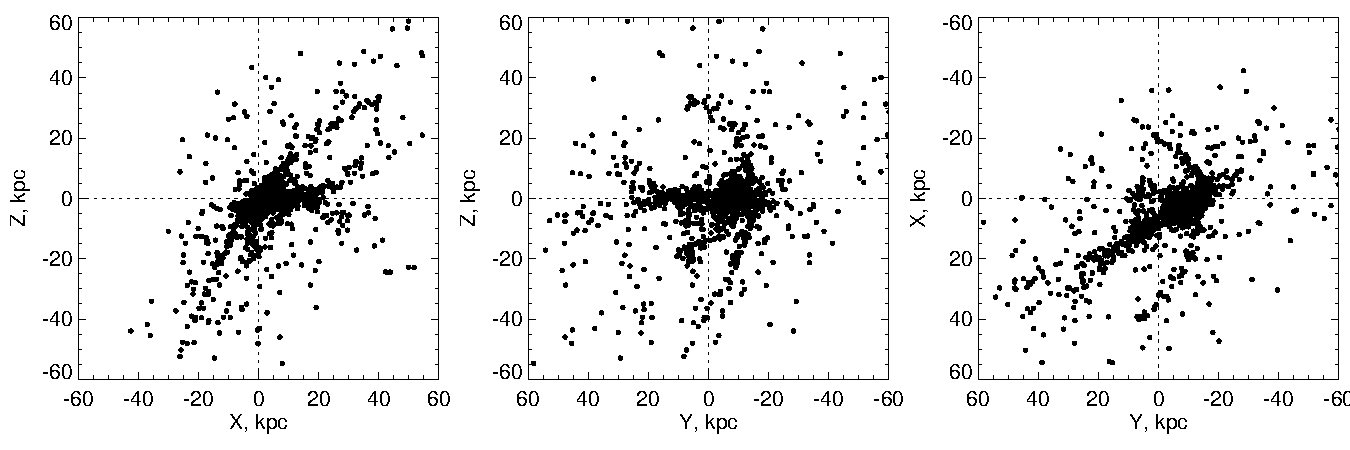
\includegraphics[width=0.95\textwidth]{orphan_paper_xyz.pdf}
  \caption[]{Galacto-centric distributions of the $\sim1,500$ \gaia
    DR2 RR Lyrae stars projected close to the OS on the sky. Only
    stars with $|\phi_2|<4^{\circ}$ and $-300<v_l <-100$, $-300<v_b
    <300$ are shown. {\it Left:} $X,Z$ plane. {\it Middle:} $Y,Z$
    plane. {\it Right:} $X,Y$ plane. Note a prominent, narrow and long
    stream-like over-density visible in all three panels.}
   \label{fig:xyzgdr2}
\end{figure*}
%


%
\begin{figure*}
  \centering
  \includegraphics[width=0.9\textwidth]{orphan_paper_selection.pdf}
  \caption[]{OS member selection. {\bf SK to provide details}}
   \label{fig:selection}
\end{figure*}
%


%
\begin{figure*}
  \centering
  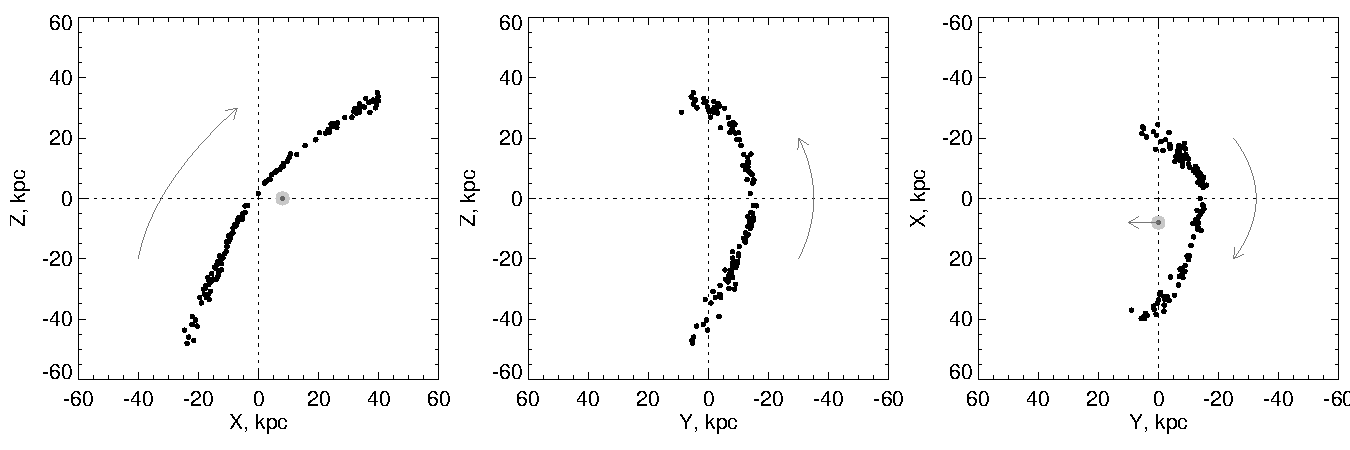
\includegraphics[width=0.97\textwidth]{orphan_paper_xyz_members.pdf}
  \caption[]{Same as Figure~\ref{fig:xyzgdr2} but limited to likely OS
    members (see Figure~\ref{fig:selection} and main text for
    details). Long curved arrow shows the direction of motion of the
    OS, while the short straight arrow indicates the motion of the Sun
    (shown as grey filled circle at $(X,Y,Z)=(8,0,0)$.}
   \label{fig:xyzmem}
\end{figure*}
%

\section{Orphan Stream with \gaia DR2 RR Lyrae}

We select a high-purity all-sky sample of RR Lyrae candidate stars
from two separate source catalogues released as part of the \gaia DR2
\citep[][]{Prusti2016, Brown2018}. More precisely, tables
\texttt{vari\_classifier\_result} and \texttt{vari\_rrlyrae}
\citep[see][]{Clementini2018,Holl2018} are joined, removing the
duplicates, and the stellar astrometry and photometry are obtained
from the main \texttt{gaia\_source} catalogue. We have culled
potential interlopers requiring \textit{phot\_bp\_rp\_excess\_factor}
to be less than 3 and have assumed $A_G=2.27$ and $M_G=0.64$ for the
extinction coefficient and the RRL absolute magnitude in the \Gaia's
$G$ band respectively \citep[see][for further
  details]{Iorio2018}. Additionally, we have assumed the Sun's
distance from the Galactic center of 8 kpc, the Local Standard or Rest
(LSR) of 235 km s$^{-1}$ and the Sun's peculiar motion as given in
\citet{LSR}.

To select the likely OS members, we translate the stellar celestial
coordinates in equatorial system $(\alpha, \delta)$ into a new
coordinate system $(\phi_1, \phi_2)$ aligned with the stream
\citep[see e.g.][]{Koposov2010}. More specifically, based on the OS
detections reported in \citet{OS_V, OS_C, Newberg2010}, we use a great
circle with a pole at $(\alpha_{\rm OS}, \delta_{\rm
  OS})=(70.5^{\circ}, -13^{\circ})$. The origin of this stream's
coordinate system is chosen to be at $(\alpha_0,
\delta_0)=(188^{\circ}, -63^{\circ})$, near the position of the OS's
crossing of the Galactic disc. Finally, $\phi_1$ increases in the
direction of the stream's motion. Several attempts at the OS kinematic
characterization can be found in \citet{Newberg2010} and
\citet{Sohn2016}. Given the OS's line-of-sight velocity and the
HST-based proper motions, we notice that the stream's velocity
component along the Galactic longitude $v_l$ remains negative
irrespective of the debris position on the sky, i.e. the stream is in
prograde motion with respect to the Galactic rotation. Accordingly, we
explore the distribution of the possible OS members selected with the
following simple cuts.

%
\begin{equation}
  \begin{aligned}
    |\phi_2| &< 4^{\circ}\\
    -300<v_l &<-100\\
    -300<v_b &<300
  \end{aligned}
\end{equation}
%

Figure~\ref{fig:xyzgdr2} shows the distributions of $\sim$1,500 RRL
stars selected with the above cuts in Galacto-centric coordinates
$X,Y$ and $Z$; here $X$ points to the Galactic anti-center and the Sun
is at $(X,Y,Z)=(8,0,0)$. A long and narrow arc or RRL stars is visible
in all three projections, crossing the Galaxy from the North (where it
is seen at $Z>0$ and $X>0$) to the South (where the signal is ar $Z<0$
and $X<0$). The stream spans a gigantic $\sim$100 kpc, traveling in
almost uninterrupted fashion through the Milky Way, coming as close as
$\sim$15 kpc to its center and reaching as far as $\sim$50 kpc into
the halo. While the Northern portion of the stream had been seen
before with SDSS and PS1, the view of its Southern Galactic section
uncovered here with \gaia DR2 is entirely new.

We can further clean the OS membership by looking closely at the
behavior of the RRL stars close to the equator of the stream's
coordinate system. To this end, Figure~\ref{fig:selection} shows the
distribution of RR Lyrae as a function of the along-stream coordinate
$\phi_2$. As the top panel of the Figure illustrates, the stream spans
some $\sim200^{\circ}$ in $\phi_1$ while exhibiting a slight bend of
several degrees in $\phi_2$. The heliocentric distance of the Orphan
debris changes slowly within $-50^{\circ}<\phi_1<50^{\circ}$, but
beyond that, the stream appears to shoot rapidly to large distances,
reaching $\sim50$ kpc on either end. Finally, a clear kinematic
pattern is visible in the bottom panel of Figure~\ref{fig:selection},
where the stream $\mu_{\phi,1}$ proper motion arches up to $\sim$4 mas
year$^{-1}$ around $\phi_1\sim40^{\circ}$ from values close to $\sim0$
mas year$^{-1}$ near the tips of the stream. Note that in all three
projections, the width of the stream also changes as a function of
$\phi_1$. Some of this variation may be due to the intrinsic evolution
of the debris density along the stream \citep[see e.g.][]{stray}, but
much of it may plausibly be associated with the change in the
measurement quality. As the stream moves away from the Sun at high
values of $|\phi_1|$, the associated errors in distance and proper
motion grow quickly, increasing the scatter around the stream's
centroid. 

Each panel of Figure~\ref{fig:selection} shows a sample of stars
selected after applying the polynomial masks from the other two panels
(the masked areas are highlighted in pale blue in each panel). The
boundaries of the masks are chosen to wrap around the bulk of the
stream's debris in a smooth and continuous manner. More precisely, the
masks are drawn as follow {\bf SK to explain}. The parameters of the
polynomials used for the stream selection are given in table XXX. {\bf
  SK to supply}. Applying all three masks shown in the Figure yields
the total of NNN OS candidate members. Table YYY lists all RRL stars
identified using the procedure described above together with their
positional and kinematic measurements from GDR2. {\bf Table
  needed}.

Figure~\ref{fig:xyzmem} is a companion to Figure~\ref{fig:xyzgdr2} as
it also shows the Galacto-centric positions of the \gaia RR Lyrae
stars, but now only those selected using the masks described
above. Left panel of the Figure emphasizes the high eccentricity of
the OS as the stream appears high stretched in this
projection. Noticeable in the middle and right panels of the Figure is
the change in the stream's curvature between the Southern and the
North Galactic hemispheres. The view of the OS in other phase-space
projections can be found in Figure~\ref{fig:memother}.

Top left panel of the Figure presents the on-sky positions of the
likely OS members in the stream-aligned coordinate system. Immediately
apparent is the striking change of the stream curvature around
$\phi_1\sim20^{\circ}$ - immediately after the stream re-emerges after
passing through the Galactic disc - where the debris behavior changes
from gently slopping down to sharply rising up in
$\phi_2$. Additionally, in the Northern end of the stream, at
$\phi_1\sim100^{\circ}$ there appears to be a curious hook
downwards. There exists a corresponding change in the debris
kinematics. For example, proper motion components $\mu_{\alpha}$ and
$\mu_{\delta}$ also show a switch in the gradient as a function of
$\phi_1$ around $\phi_1\sim20^{\circ}$. Note, however that the
evolution of the physical velocity components $v_l$ and $v_b$ (and
also $v_{\phi,1}$ and $v_{\phi,2}$) is considerably
smoother. Therefore, some of the change in the proper motions (shown
in the second row from the top) is due to the change in the
line-of-sight distance.

%
\begin{figure*}
  \centering
  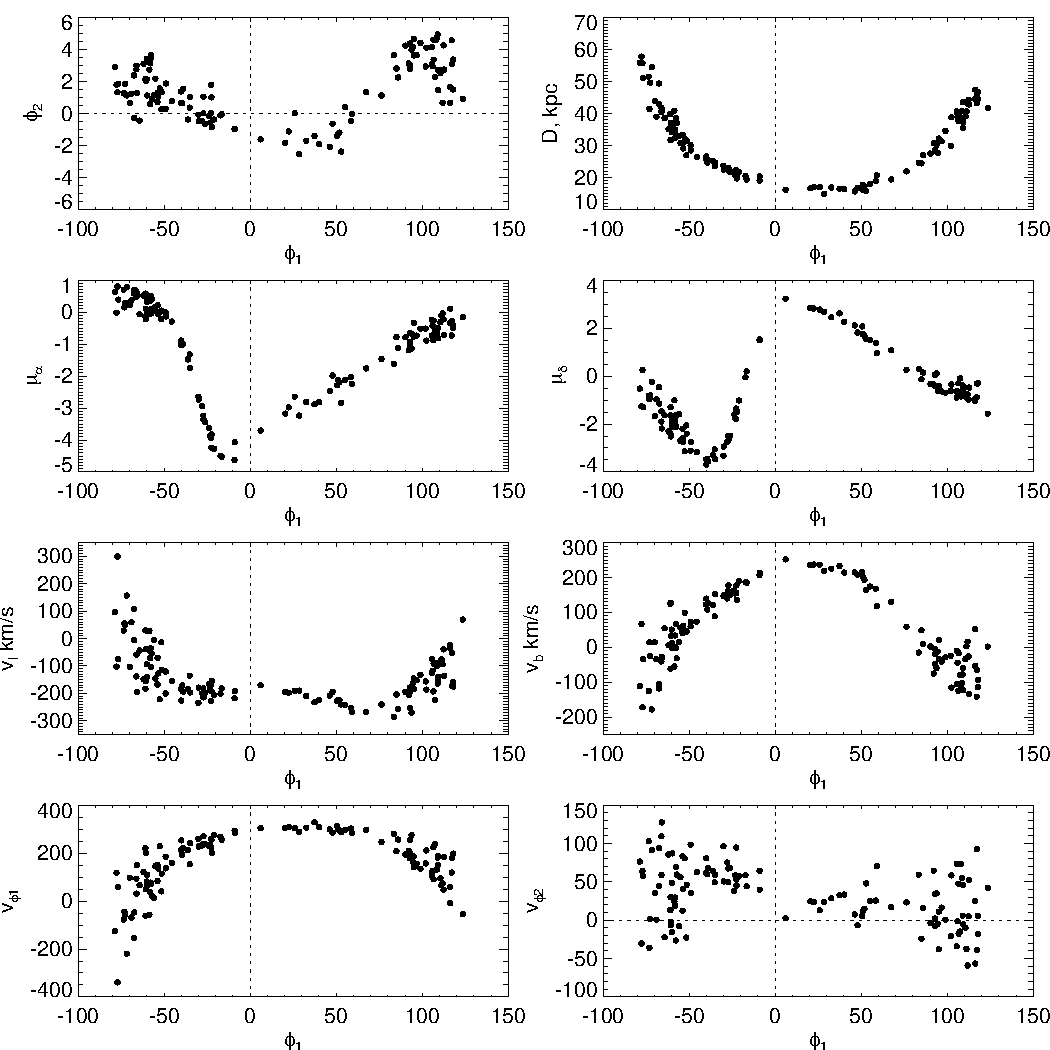
\includegraphics[width=0.9\textwidth]{orphan_paper_phi1_members.pdf}
  \caption[]{Phase-space projections of the likely OS member RR Lyrae
    as a function of the stream longitude $\phi_1$. {\it Top left:}
    Positions of the OS stars on the sky in the stream-aligned
    coordinates $\phi_1, phi_2$. {\it Top right:} Heliocentric
    distance as a function of $\phi_1$. {\it Second row, left:} RA
    component of proper motion $\mu_{\alpha}$. {\it Second row,
      right:} Dec component of proper motion $\mu_{\delta}$. {\it
      Third row, left:} Velocity component along Galactic longitude
    $v_l$. {\it Third row, right:} Velocity component along Galactic
    latitude $v_b$. {\it Bottom left:} Along-stream velocity
    $v_{\phi,1}$. {\it Bottom right:} Across-stream velocity
    $v_{\phi,2}$.}
   \label{fig:memother}
\end{figure*}
%

\section{OS with giants in \gaia and DECaLS}


\section*{Acknowledgments}

We thank Michael for illuminating discussions. The research leading to
these results has received funding from the European Research Council
under the European Union's Seventh Framework Programme (FP/2007-2013)
/ ERC Grant Agreement n. 308024. This research was started at the NYC
Gaia DR2 Workshop at the Center for Computational Astrophysics of the
Flatiron Institute in April 2018 and made use of data from the
European Space Agency mission Gaia (http://www.cosmos.esa.int/gaia),
processed by the Gaia Data Processing and Analysis Consortium (DPAC,
http://www.cosmos.esa.int/web/gaia/dpac/consortium). Funding for the
DPAC has been provided by national institutions, in particular the
institutions participating in the Gaia Multilateral Agreement.

\bibliography{references}

\label{lastpage}

\end{document}

